\section{Result}

\newcommand{\e}[1]{\times 10^{#1}}

The frequency we read from the signal generator is $f=34498 \pm 1$Hz. The
temperature is $23 \pm 1 ^\circ C$.

\subsection{Measurements for resonance method}

The measurements are shown in Table~\ref{data_res} with the calculation for $L_{10+i}-L_i$.


\begin{table}[H] \small
    \centering
    \begin{tabular}{|c|c|c|c|c|c|}
    \hline
        \multicolumn{2}{|c|}{$L_i[\times 10^{-3} m]\pm[0.01\times 10^{-3} m]$} & 
        \multicolumn{2}{|c|}{$L_i[\times 10^{-3} m]\pm[\times 10^{-3} m]$} &
        \multicolumn{2}{|c|}{$L_{10+i}-L_i[\e{-3}m]$}\\\hline
        1  & 29.37 & 11 &  80.44 & 1  & 51.07 \\\hline
        2  & 34.49 & 12 &  85.48 & 2  & 50.99 \\\hline
        3  & 39.60 & 13 &  90.01 & 3  & 50.41 \\\hline
        4  & 44.74 & 14 &  95.65 & 4  & 50.91 \\\hline
        5  & 49.83 & 15 & 100.82 & 5  & 50.99 \\\hline
        6  & 54.90 & 16 & 105.93 & 6  & 51.03 \\\hline
        7  & 60.06 & 17 & 111.12 & 7  & 51.06 \\\hline
        8  & 65.24 & 18 & 116.20 & 8  & 50.96 \\\hline
        9  & 70.37 & 19 & 121.32 & 9  & 50.95 \\\hline
        10 & 75.38 & 20 & 126.39 & 10 & 51.01 \\\hline
    \end{tabular}
    \caption{Data for the resonance method}\label{data_res}
\end{table}

The average value of $\Delta L$ is calculated  based on the results presented in Table \ref{data_res} as

\[
    \overline{\Delta L}=\frac{1}{10}\sum_{i=1}^{10}\Delta L_i=(50.94\pm 0.05)\times 10^{-3} m,\quad u_{r,\Delta}=0.10\%.
\]

Hence, the wavelength $\lambda$ can be calculated as

\[
        \lambda=\frac{2\Delta L}{n}=\frac{2\times50.94\times 10^{-3} }{10}=(10.19 \pm0.01)\times 10^{-3} m,\quad u_{r,\lambda}=0.10\%.
\]

The speed of sound in air $v$ is

\[
    v= 351.45 \pm 0.4 m/s,\quad u_{r,v}=0.11\%.
\]

\subsection{Measurements for phase comparison method}

The measurements are shown in Table \ref{data_pha} with the calculation for $L_{6+i}-L_i$.

\begin{table}[H] \small
    \centering
    \begin{tabular}{|c|c|c|c|c|c|}
    \hline
        \multicolumn{2}{|c|}{$L_i[\times 10^{-3} m]\pm[0.01\times 10^{-3} m]$} & 
        \multicolumn{2}{|c|}{$L_i[\times 10^{-3} m]\pm[0.01\times 10^{-3} m]$} &
        \multicolumn{2}{|c|}{$L_{6+i}-L_i[\e{-3}m]$}\\\hline
        1 & 54.00 & 7 & 113.41 & 1 & 59.41 \\\hline
        2 & 64.06 & 8 & 122.04 & 2 & 57.98 \\\hline
        3 & 72.97 & 9 & 131.76 & 3 & 58.79 \\\hline
        4 & 81.02 & 10 & 141.83 & 4 & 60.81 \\\hline
        5 & 91.17 & 11 & 153.65 & 5 & 62.46 \\\hline
        6 & 103.49 & 12 & 163.08 & 6 & 59.59 \\\hline
    \end{tabular}
    \caption{Data for the phase comparison method}\label{data_pha}
\end{table}
    
The average value of $\Delta L$ is calculated  based on the results presented in Table \ref{data_res} as

\[
    \overline{\Delta L}=\frac{1}{6}\sum_{i=1}^{6}\Delta L_i=(59.84\pm 1.7)\times 10^{-3} m,\quad u_{r,\Delta L}=3\%.
\]

Hence, the wavelength $\lambda$ can be calculated as

\[
    \lambda=\frac{\Delta L}{n}=\frac{\times59.84\e{-3}}{6}=(9.973\pm0.3)\times 10^{-3} m,\quad u_{r,\lambda}=3\%.
\]

The speed of sound in air $v$ is

\[
v=348.95\pm10 m/s,\quad u_{r,v}=3\%.
\]

\subsection{Measurements for time difference method (liquid)}

We obtain the speed of sound in water from Table \ref{data_tim} by linear fitting (See Figure \ref{lt}).
    
\begin{table}[H] \small
    \centering
    \begin{tabular}{|c|c|c|c|c|}
    \hline
        & $t_i[\e{-6}s]$ & $u_{t_i}[\times 10^{-6} s]$ & $L_i[\times 10^{-3} m]$ & $u_{L_i}[\times 10^{-3} m]$\\\hline
        1 & 159.6 & 0.2 & 230.00 & 0.01\\\hline
        2 & 154.4 & 0.2 & 220.00 & 0.01\\\hline
        3 & 148.2 & 0.2 & 210.00 & 0.01\\\hline
        4 & 141.8 & 0.2 & 200.00 & 0.01\\\hline
        5 & 134.0 & 0.2 & 190.00 & 0.01\\\hline
        6 & 128.0 & 0.2 & 180.00 & 0.01\\\hline
        7 & 121.4 & 0.2 & 170.00 & 0.01\\\hline
        8 & 114.4 & 0.2 & 160.00 & 0.01\\\hline
        9 & 108.0 & 0.2 & 150.00 & 0.01\\\hline
        10 & 101.6 & 0.2 & 140.00 & 0.01\\\hline
        11 & 94.8 & 0.2 & 130.00 & 0.01\\\hline
        12 & 87.8 & 0.2 & 120.00 & 0.01\\\hline
    \end{tabular}
    \caption{Data for Figure \ref{lt}}\label{data_tim}
\end{table}
\begin{figure}[H]
    \centering
  %  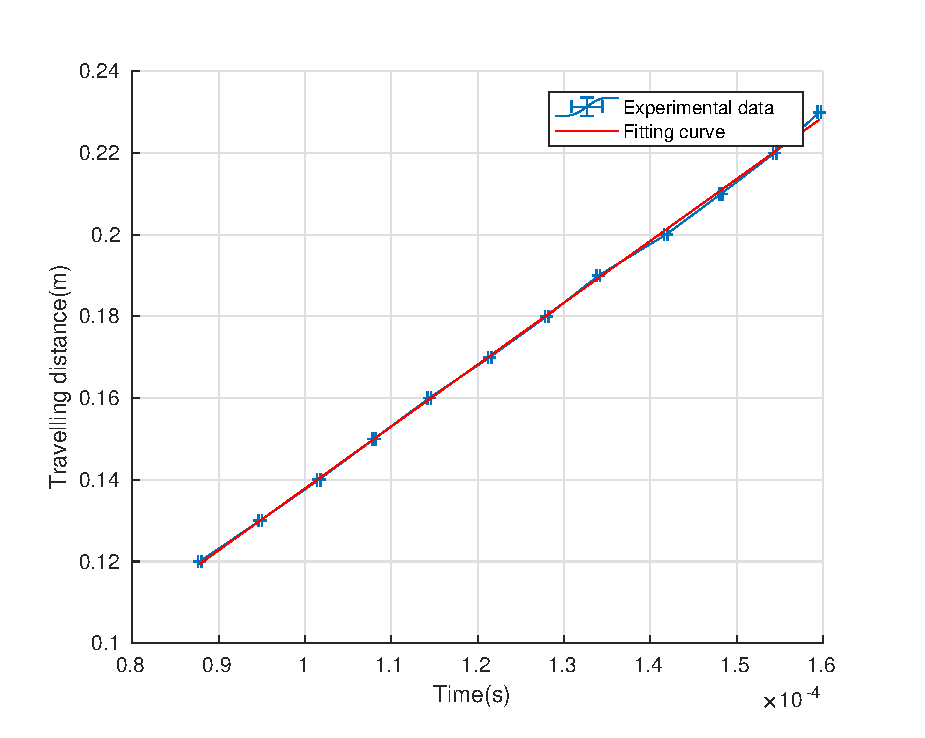
\includegraphics[height=10cm]{images/lt.eps}
    \caption{Fitting curve for $L\ vs.\ t$. (The errorbar is relatively \textbf{small})}\label{lt}
\end{figure}
\begin{figure}[H]
    \centering
    %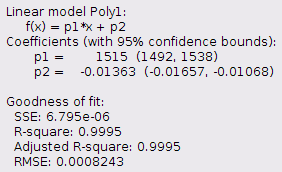
\includegraphics[height=6cm]{images/ltinfo.png}
    \caption{Information for Fitting curve in Figure \ref{lt}}\label{ltinfo}
\end{figure}

From the data processing of Matalb we know about the slope that 
\[
    v_{water}=1515\pm20m/s.
\]